\begin{figure}
  \centering
  \begin{subfigure}[b]{0.33\textwidth}
    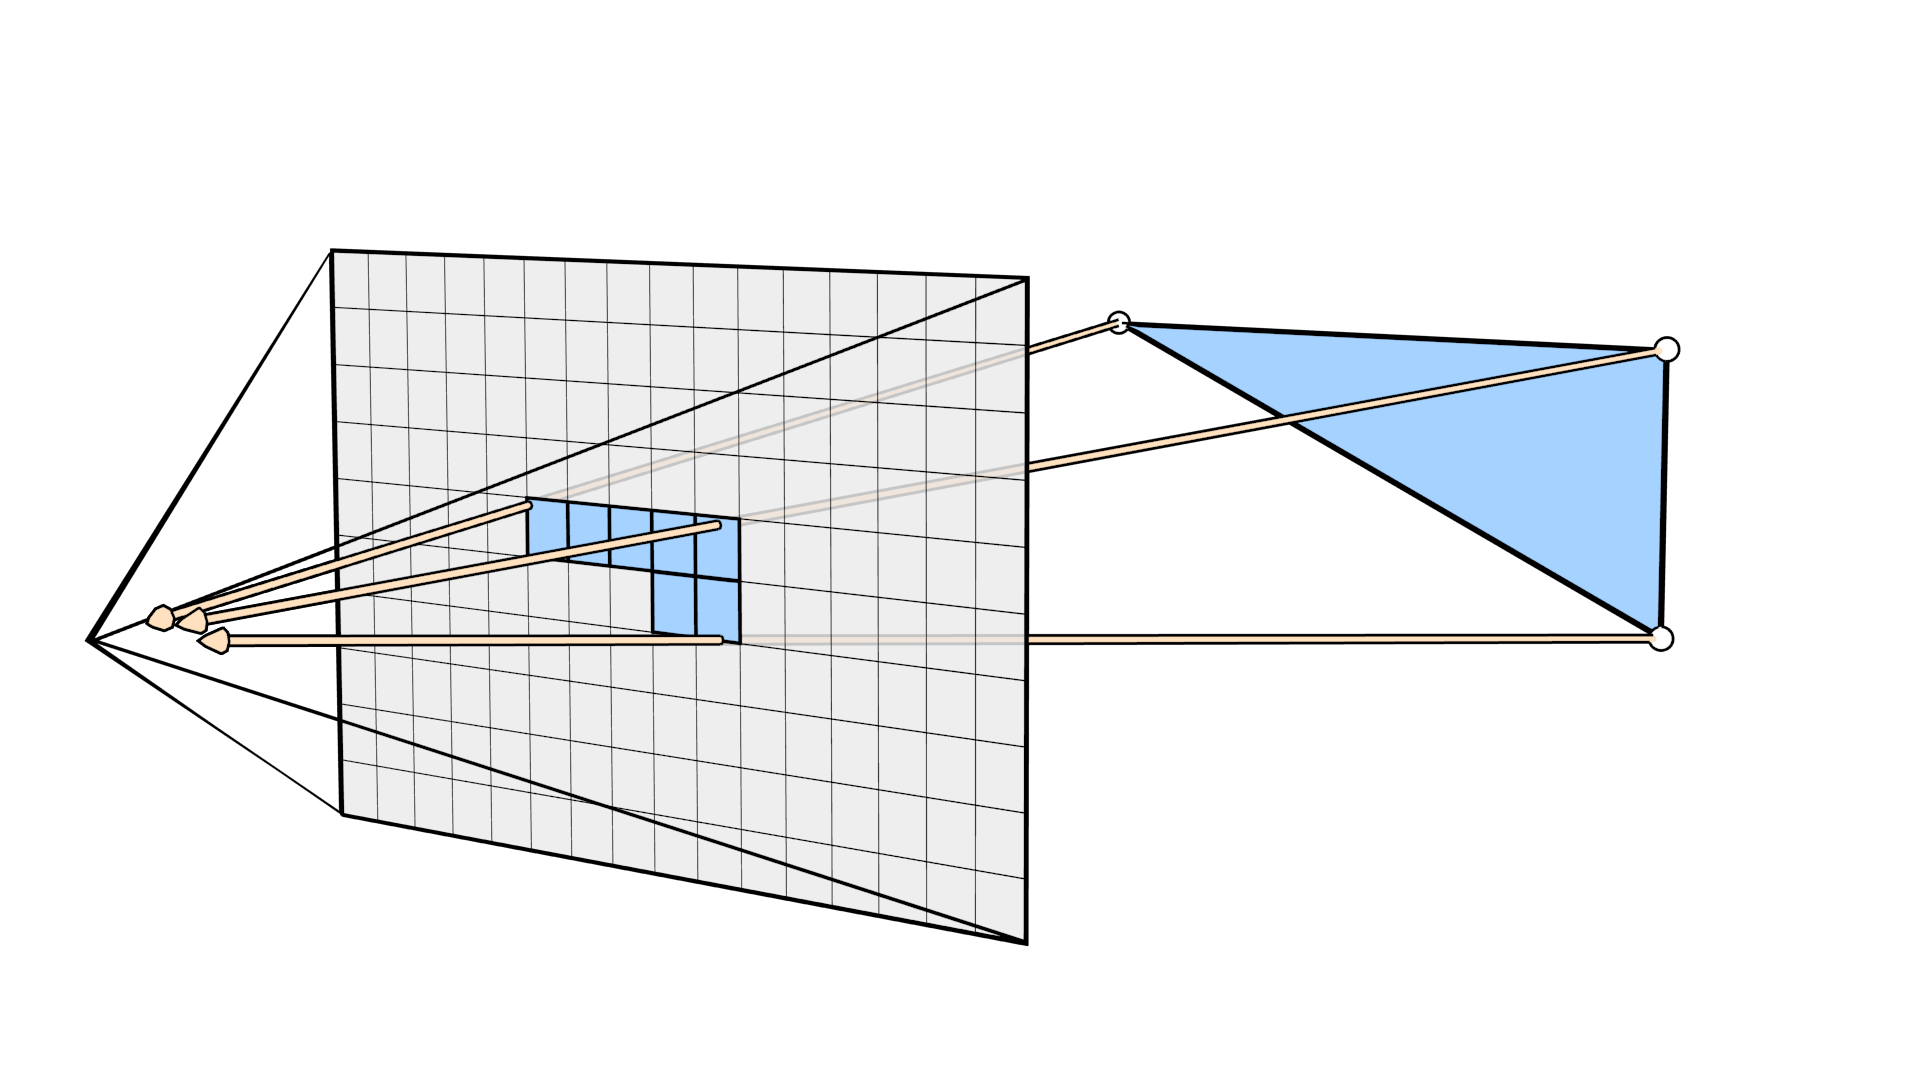
\includegraphics[width=\textwidth]{./img/raw/rs-rasterisatie/rasterisation1.png}
    \caption{Perspectiefprojectie.}
    \label{fig:rs-rasterisatie:1}
  \end{subfigure}%
  \begin{subfigure}[b]{0.33\textwidth}
    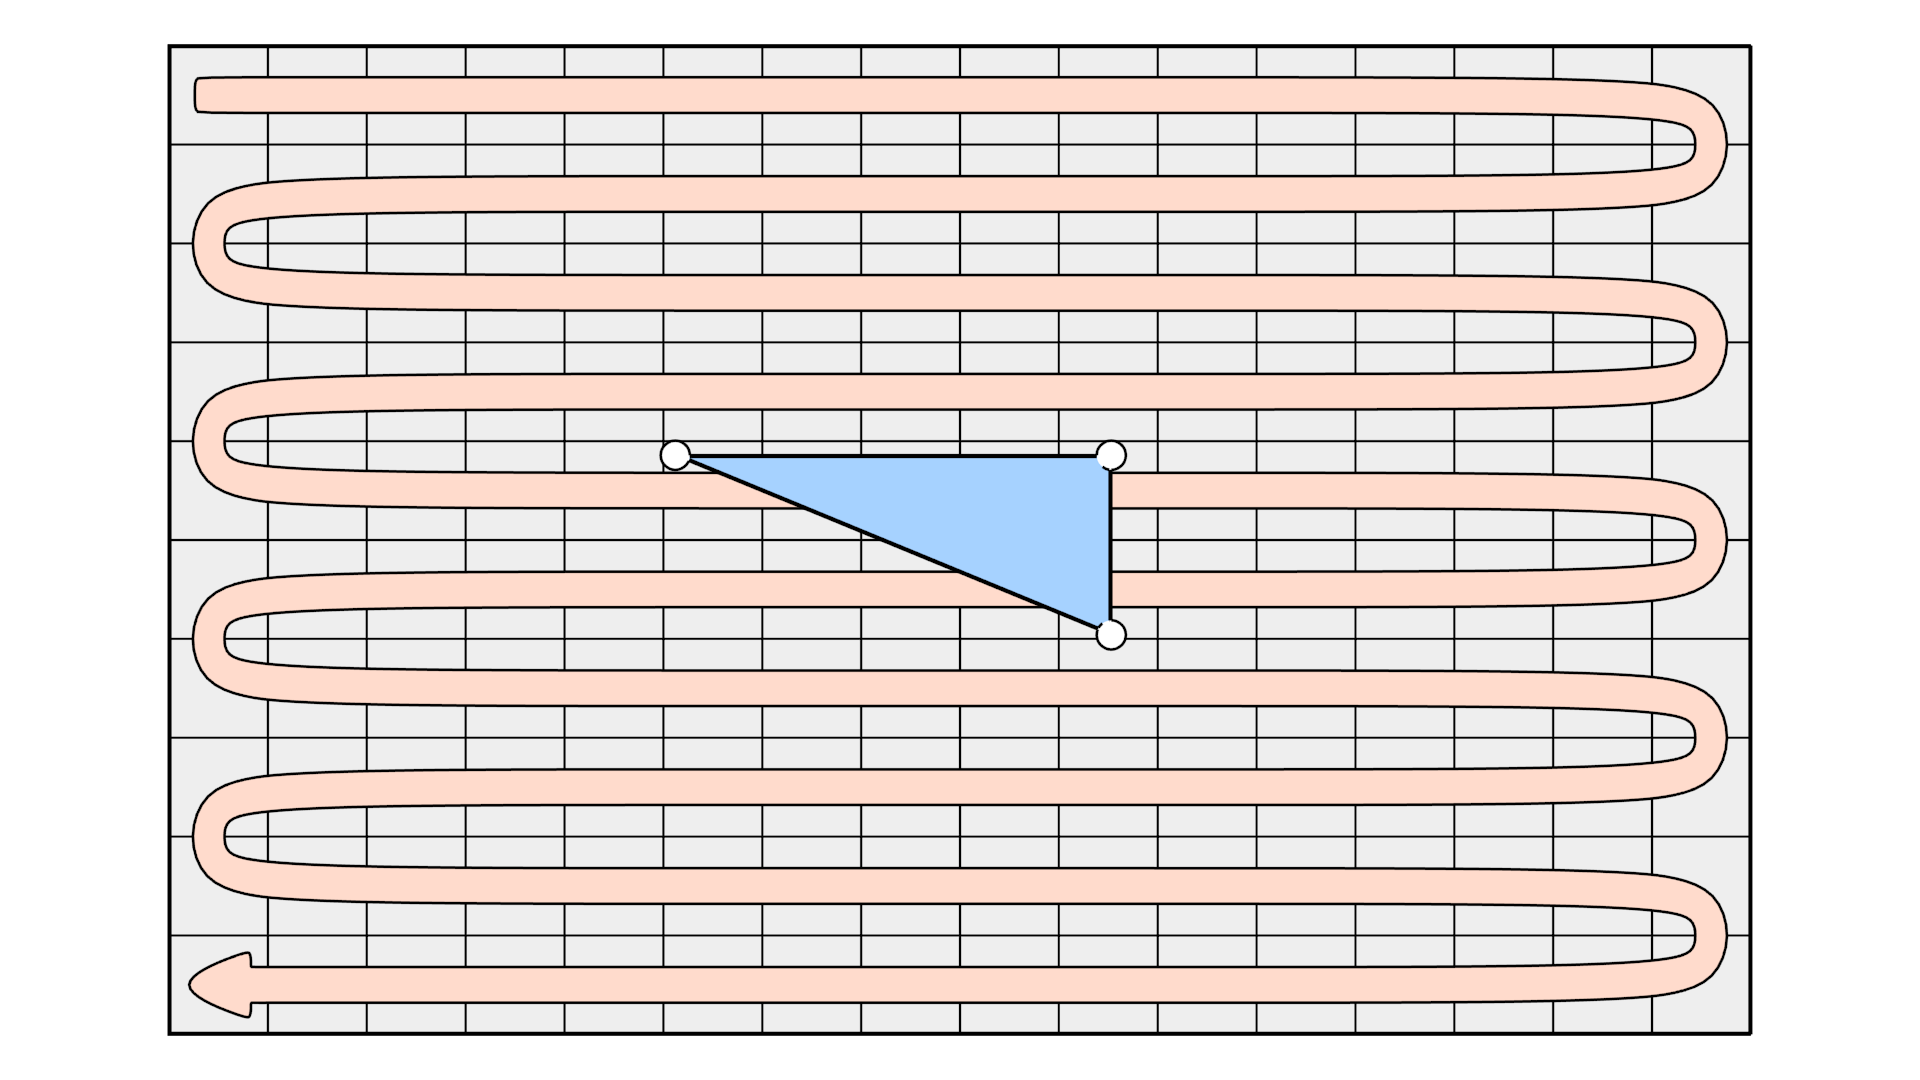
\includegraphics[width=\textwidth]{./img/raw/rs-rasterisatie/rasterisation2.png}
    \caption{Pixeloverloping.}
    \label{fig:rs-rasterisatie:2}
  \end{subfigure}%
  \begin{subfigure}[b]{0.33\textwidth}
    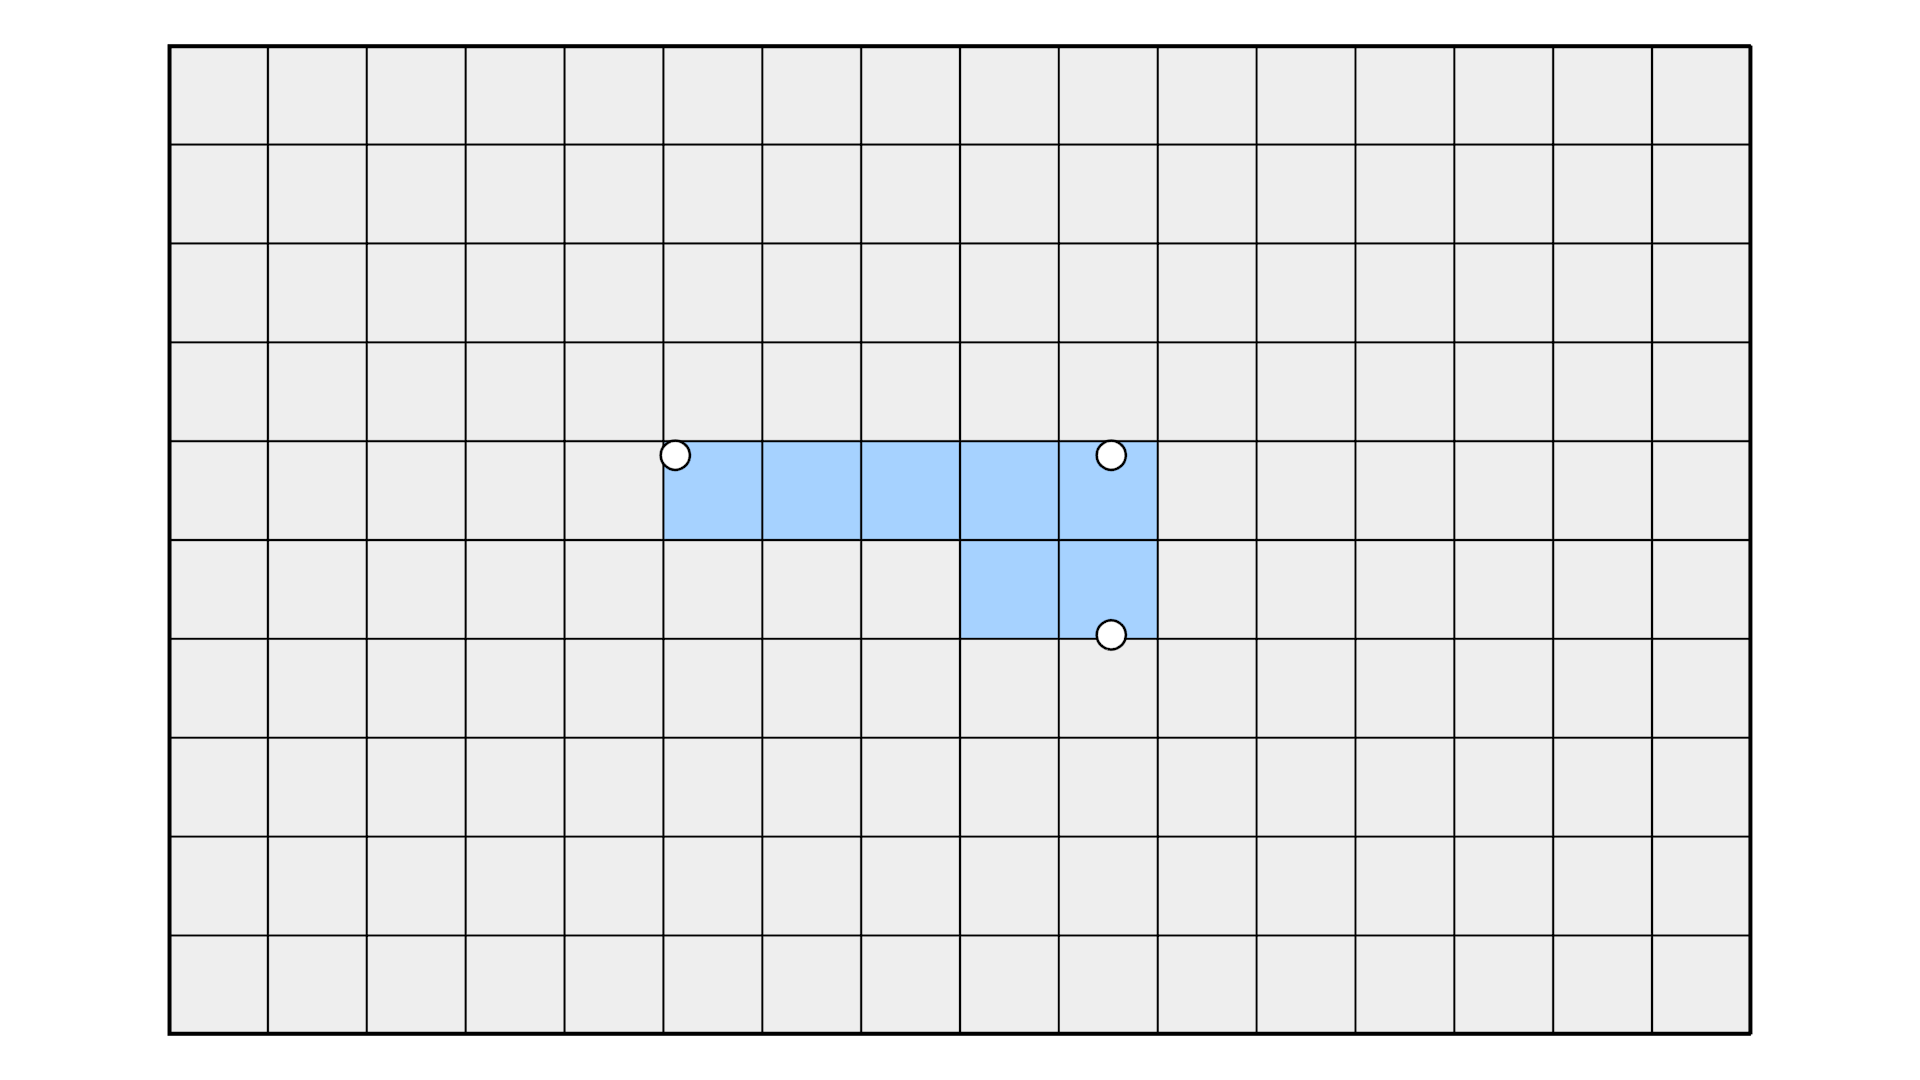
\includegraphics[width=\textwidth]{./img/raw/rs-rasterisatie/rasterisation3.png}
    \caption{Pixeltoekenning}
    \label{fig:rs-rasterisatie:3}
  \end{subfigure}%
  \caption{Het rasterisatie algoritme.}
  \label{fig:rs-rasterisatie}
\end{figure}
